
\section{Discussion}\label{chap:discussion}

%Discuss the results. What is the outcome of your experimetns?
This subsection shortly discusses the empirical results and then extensively compares the findings of this work to the existing literature while trying to explain some differences. It is followed by a subsection describing the limitations and possible extensions of this work. This subsection is concluded by the problems we encountered during the implementation so others can avoid them in the future.

\subsection{Our work}
This subsection discusses our findings, first we will analyze how input shuffling could influence the learning rate and conclude with the discussion of unexpected results.

\subsubsection{Shuffling and learning rate with SGD}
When the model used SGD as an optimizer it was able to use higher learning rates when input shuffling was used, as shown in figures \ref{fig:results_sgd}, \ref{fig:results_mom} and \ref{fig:results_nag} Therefore arises the questions why these phenomena happen, especially as it did not happen with advanced optimizers. One possibility is the use of the batched version of the SGNS. In consequence, when the input is not shuffled the same word will often appear in one batch, hence the optimizer is presented with an average value of the gradient, which can be imprecise. This is counter-attacked by advanced optimizers as they have adaptive learning rates, i.e a frequent appearing feature will have a low learning rate.

\subsubsection{Large differences with NAG and SGD when using shuffling}
SGD and NAG both have very different values when using shuffling in comparison to unshuffled input, as shown in figures \ref{fig:results_sgd} and \ref{fig:results_nag}, plain SGD. We do not only attribute those results to input shuffling but partially also to a good random initialization guess. Due to a lack of time these results were not replicate more than once.

\subsection{Comparison to Gensim}
This subsection will compare our finding extensively to Gensim \cite{gensim}. As explained in Section \ref{ssec:gensim}, Gensim is optimized to have a very high throughput, this made it possible to achieve a lot of computations. Furthermore, Gensim provides access to the loss and the resulting word embeddings, which facilitated the comparison process.

\iffalse
As Mikolov et al. published the original paper which introduced the SGNS, it is, of course, relevant to compare ourselves to their work. The first important thing to take under account is that Mikolov et al. only trained their model on a very large google news dataset incorporating more than 3 billion words. This makes the comparison of our work more difficult. But we will make some assumptions, as they could be of value if true.
In their original paper, Mikolov et al. reported results from computations that took 1 and 3 epochs. We accord these good results, which clearly outperformed our SGD model and Gensim, to the very large dataset and furthermore, as a matter of fact, their results are better with 3 than with 1 epoch. We do not have any information about the convergence time or criterion. Hence it would be interesting to use their dataset for comparison. \\
One thing we can compare is the quality of our word embeddings. Mikolov et al. did not report any results on their model with the text8 dataset, but they, therefore, published their code. Which was then used by Ji et al \cite{intel} and they tested the model on the text8 dataset. They reported a word similarity of 0.63 on the word similarity task. This is obviously outperformed by all our models. We did not find any explanation on why those results differ as much. \\
The final assumption is that an advanced optimizer could maybe outperform SGD in terms of quality on a large data set. This will be discussed in further work.

\fi

\subsubsection{Configuration of Gensim}
The training with Gensim has a lot of possible parameters an extended list can be found in the appendix. This subsection will only describe the parameters we changed from the default setting. The description of each parameter has the following form: \\
\texttt{name} (type) -- \textit{Description} -- Value\\
Parameters:
\begin{itemize}
\item \texttt{sentences} (iterable of iterables) -- \textit{Dataset} -- text8 document splitted into sentences of 20 words
\item \texttt{size}(int) – \textit{Dimensionality of the word vectors } -- 100
\item \texttt{window} (int) --\textit {Maximum distance between the current and predicted word within a sentence }-- 5
\item \texttt{min\_count }(int) --\textit{ Ignores all words with total frequency lower than this }-- 5
\item \texttt{workers} (int) -- \textit{ Number of threads used to train the model} -- 4
\item \texttt{sg} ({0, 1}) --\textit{ Training algorithm: 1 for skip--gram}--1
\item \texttt{negative} (int) --\textit{Number of negative samples}-- 10
\item \texttt{ ns\_exponent} (float) --\textit{ Exponent in the unigram distribution, when choosing random samples, as shown in Equation \ref{eq:unigram} }-- 0.75
\item \texttt{alpha} (float) --\textit{ The initial learning rate. }-- 0.025
\item \texttt{min\_alpha} (float) --\textit{ Learning rate will linearly drop to min\_alpha as training progresses }--0.0001
\item \texttt{sample} (float) --\textit{ Treshold for subsampling as described in Equation \ref{eq:sampling}} -- 1e--4
\item \texttt{iter} (int) --\textit{ Number of iterations (epochs) over the corpus. }-- 10
\
\item \texttt{compute\_loss} (bool) --\textit{If True, loss is stored at the end of each batch}-- True
\item \texttt{callbacks} (iterable of CallbackAny2Vec) --\textit{ Set of functions executed in order to follow the loss and the progress of the model in word similarity }-- see Appendix
\end{itemize}

\subsubsection{Gensim vs. SGD}
As stated earlier, we are not going to compare this work to Gensim in run time. Gensim is heavily optimized and written in cython\footnote{https://rare-technologies.com/word2vec-in-python-part-two-optimizing/}, which is 23x faster than plain Numpy. Since we used PyTorch the difference is not that big, but still remains. As shown in Figure \ref{fig:gensim_vs_adam} the convergence time was not the same between our implementation and Gensim. There are different possible reasons why this could be the case:\\ First, our batched approach could hinder performance in terms of convergence since our loss function is not exactly the same. When a word appears more than once in our batch, the gradient will be an average over the gradients of each pair alone, as it is done by Gensim.\\ Secondly, a difference to our implementation is the fact that Gensim checks whether negative samples are not equal to the context word. If that is the case Gensim selects a new random sample. Therefore, the learning of the input and output context is optimized. \\Finally, another possibility is the decay of the learning rate used by Gensim. In fact, decaying the learning rate has been proven in a lot of work to decrease the convergence time. Gensim linearly decreases the learning rate, as we did not use this technique, the decay of the learning rate could help explain the noted differences. \\ The first hypothesis, the fact that we used a batched approach, may be confirmed by the fact that when combined with input shuffling SGD does perform closer to Gensim, going from 11 to 7 epochs to converge, as input shuffling reduces the number of co-occurrence of the same word in a batch.
Now the question arises if the 3 epochs, that Gensim is better, can be explained by the selection of better negative samples and the learning rate decay?

\subsubsection{Gensim vs. Adam}
The Adam optimizer did outperform the Gensim application in quality of word embeddings (only slightly: 0.01 correlation coefficient better) and convergence time. Adam converged in 2 epochs while Gensim in 4. To confirm the achieved results we ran each computation 40 times. The results can be seen in Figure \ref{fig:gensim_vs_adam}.

\begin{figure}[h]
\centering
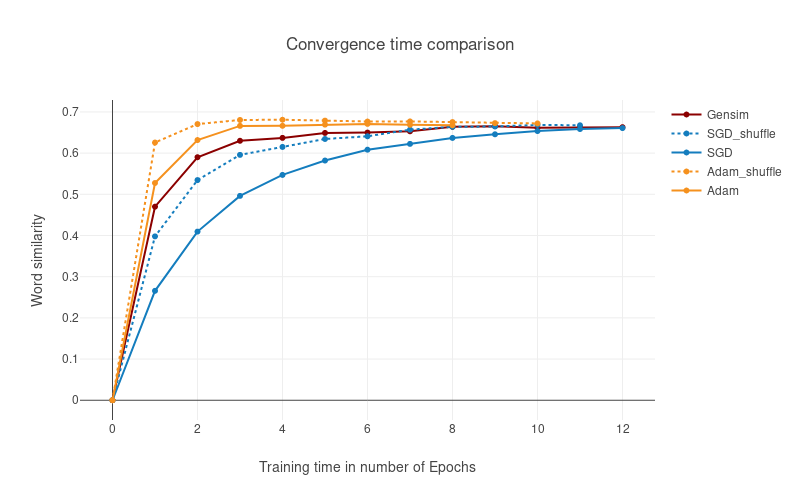
\includegraphics[scale=0.45]{images/gensim_vs_adam}
\caption{Convergence time of SGD and Adam compared to Gensim}
\label{fig:gensim_vs_adam}
\end{figure}\subsection{Challenges faced}
During our implementation we did encounter some problems, this subsection has the purpose of preventing the scientific community from making the same mistakes.
\subsubsection{Using the wrong embeddings}
To start with, we did not choose the same initialization value as Gensim in our word embeddings. We initialized the projection layer with a normal distribution between (-1,1), as opposed to Gensim which initializes all the weights to 0. The reason for this, is that at the beginning of our experiments we did not achieve good results with the same initialization as Gensim. Retrospectively we accord this to a learning rate that was too low. After a few simulations, we saw that we did not perform as good as Gensim. And as we changed the initialization of the projection layer back to 0, and already had adjusted the learning rate, we achieved good results. Therefore, this is a recommendation to future work to not set the initialization to (-1,1).

\subsubsection{Batch size and loss function adjustements}\label{ssec:bs_lf}
During our experiments, we faced a moment where we needed to us a very high learning rate (50) to achieve good results. As this is the complete opposite of what is standard we made a few changes to remedy the problem.\\
First, we needed to find a good batch size. During the above-explained raise of the learning rate, we used a batch size of 5000. We then decided to take a batch size of 2000.\\
Secondly, at the same time, we did experiment with different loss functions. As our batched model does not have exactly the same loss function as introduced by Mikolov et al. \cite{mikolov}, we needed to find one that suited our goals the best. At the beginning of our experiment, we took the average of all the scores stored in our final matrix, as explained in \ref{ssec:b_SGM}. But then chose to take the sum as the training did not seem optimal.\\
With these two changes, we did increase convergence time and word similarity, while at the same time having a usual learning rate. \\
Know the question arises why this happened? Is this because of the shape of the loss function better suits our advanced optimizers? Or because the loss function is closer to its original form? Our hypothesis looks the following way:
When taking the average, our loss function is represented as follows:
\begin{equation}
\frac{-1}{b }* \sum_{x\in X} loss(x)
\end{equation}
where $X$ is our batch and $b = |X|$.
When taking the partial derivative of each parameter, the constant $ \frac{-1}{b }$ will remain the same. Therefore, it's the same as taking the sum as the loss function and multiplying each gradient with $\frac{-1}{b }$. As our batch size was really high, i.e 2000 and 5000, this could highly influence the learning rate. This is also the conclusion of Goyal et al. \cite{fb}, that worked with very high batch sizes, i.e 8000: "When the minibatch size is multiplied by k, multiply the learning rate by k".

\subsection{Future Work}
This work shows that the convergence time of the SGNS could be improved by using input shuffling and advanced optimizers. As with every work, there still exists possible extensions. First and foremost an aspect of our implementation that can be prejudicial is that we only extensively tested our model with one small dataset. The fact that we only used one dataset as well that it's a small one is problematic. By using a very small dataset we do not use the model in the condition it is most needed for, as the dataset used in practice usually consists of more than 1 billion words. There is a small argument that can be made for machine translation as the use of small parallel corpus is not unusual in this field. But the main issue with using only one data set it that it has been shown that some optimizers perform better with specific shapes of loss functions. To make a compelling argument it's, therefore, necessary to show that our model with the use of Input shuffling and Adam as its optimizer also outperform Gensim with other data sets, so that the claim can hold consistently, it needs to be confirmed with other datasets as well.
Furthermore, our implementation did not outperform Gensim in run time, as this was not the goal of our work. Therefore, one could improve an already existing, optimized version, with input shuffling and advanced optimizers and should achieve a better run time than Gensim.